\documentclass[convert={density=900,size=1080x800,outext=.png}, margin=5mm]{standalone}
\usepackage[utf8]{inputenc}
\usepackage{tikz}
\usetikzlibrary{calc, positioning}
\usetikzlibrary{arrows.meta}
\usetikzlibrary{matrix}
\usetikzlibrary{shadows}
\usepgflibrary{shapes.misc}
\usepgflibrary{{shapes.geometric}}
\usetikzlibrary{arrows,positioning,shapes}

\pgfdeclarelayer{shadow} 
\pgfsetlayers{shadow,main}
\def\shadowradius{3pt}


\def\lw{1mm}        % Arrow line width
\def\mw{2cm}        % Minimum width of component
\def\mh{0.75cm}     % Minimum height of component
\def\trianglecoordinate{2mm}    % Starting coordinate clock input triangle of components

\newcommand\drawshadowbis[1]{
    \begin{pgfonlayer}{shadow}
        \fill[inner color=black,outer color=white] ($(#1.south west)$) circle (\shadowradius);
        \fill[inner color=black ,outer color=white] ($(#1.north west)$) circle (\shadowradius);
        \fill[inner color=black ,outer color=white] ($(#1.south east)$) circle (\shadowradius);
        \fill[inner color=black,outer color=white] ($(#1.north east)$) circle (\shadowradius);
        \fill[ top color=black, bottom color=white] ($(#1.south west)+((0,-\shadowradius)$) rectangle ($(#1.south east)$);
        \fill[left color=black,right color=white] ($(#1.south east)$) rectangle ($(#1.north east)+((\shadowradius,0)$);
        \fill[bottom color=black,top color=white] ($(#1.north west)$) rectangle ($(#1.north east)+((0,\shadowradius)$);
        \fill[right color=black,left color=white] ($(#1.south west)$) rectangle ($(#1.north west)+(-\shadowradius,0)$);
    \end{pgfonlayer}
    }

\tikzset{
    border/.style = { 
        draw, rectangle, minimum width=0.75\mw, minimum height=\mh, very thick
    },
    pics/Component/.style ={
        code = {
            \node [border, align=center](-edge){#1};
    }}
    }

\tikzset{
    decisionborder/.style = { 
        draw, diamond,, minimum width=\mw, minimum height=0.7*\mh, very thick
    },
    pics/Decision/.style ={
        code = {
            \node [decisionborder, align=center](-decisionedge){#1};
    }}
    }


\begin{document}
    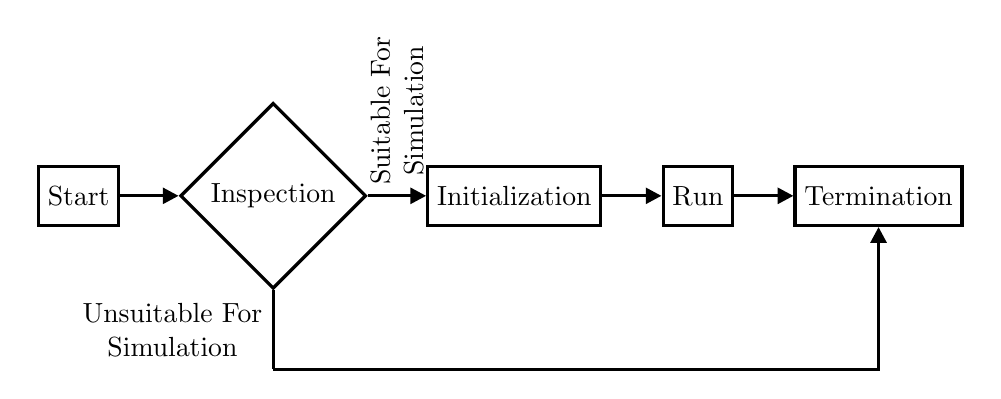
\begin{tikzpicture}
        % Place the blocks 
        \matrix (m) [matrix of nodes, ampersand replacement=\&, column sep = 0.75cm, row sep = 1cm, 
            nodes={anchor=center}]{
        \draw pic (b1) {Component={Start}}; \&
        \draw pic (b2) {Decision={Inspection}}; \&
        \draw pic (b3) {Component={Initialization}}; \&
        \draw pic (b4) {Component={Run}}; \&
        \draw pic (b5) {Component={Termination}}; \\
        };
        \begin{scope}[very thick, >={Triangle[width=2mm,length=2mm]}]
            \draw[->] (b1-edge.east) -- (b2-decisionedge.west);
            \draw[->] (b2-decisionedge.east) -- node[midway, anchor=west, align=center, rotate=90]{Suitable For\\Simulation} (b3-edge.west);
            \draw[->] (b3-edge.east) -- (b4-edge.west);
            \draw[->] (b4-edge.east) -- (b5-edge.west);
            \draw[-] (b2-decisionedge.south) -- node[midway, anchor=east, align=center]{Unsuitable For\\Simulation} ++(0cm, -1cm) coordinate(a);
            \draw[->] (a) -| (b5-edge.south);
        \end{scope}
    \end{tikzpicture}
\end{document}
